% Options for packages loaded elsewhere
\PassOptionsToPackage{unicode}{hyperref}
\PassOptionsToPackage{hyphens}{url}
\PassOptionsToPackage{dvipsnames,svgnames,x11names}{xcolor}
%
\documentclass[
  10pt,
  letterpaper,
  DIV=11,
  numbers=noendperiod]{scrartcl}

\usepackage{amsmath,amssymb}
\usepackage{iftex}
\ifPDFTeX
  \usepackage[T1]{fontenc}
  \usepackage[utf8]{inputenc}
  \usepackage{textcomp} % provide euro and other symbols
\else % if luatex or xetex
  \usepackage{unicode-math}
  \defaultfontfeatures{Scale=MatchLowercase}
  \defaultfontfeatures[\rmfamily]{Ligatures=TeX,Scale=1}
\fi
\usepackage{lmodern}
\ifPDFTeX\else  
    % xetex/luatex font selection
\fi
% Use upquote if available, for straight quotes in verbatim environments
\IfFileExists{upquote.sty}{\usepackage{upquote}}{}
\IfFileExists{microtype.sty}{% use microtype if available
  \usepackage[]{microtype}
  \UseMicrotypeSet[protrusion]{basicmath} % disable protrusion for tt fonts
}{}
\makeatletter
\@ifundefined{KOMAClassName}{% if non-KOMA class
  \IfFileExists{parskip.sty}{%
    \usepackage{parskip}
  }{% else
    \setlength{\parindent}{0pt}
    \setlength{\parskip}{6pt plus 2pt minus 1pt}}
}{% if KOMA class
  \KOMAoptions{parskip=half}}
\makeatother
\usepackage{xcolor}
\usepackage[margin=1in]{geometry}
\setlength{\emergencystretch}{3em} % prevent overfull lines
\setcounter{secnumdepth}{5}
% Make \paragraph and \subparagraph free-standing
\makeatletter
\ifx\paragraph\undefined\else
  \let\oldparagraph\paragraph
  \renewcommand{\paragraph}{
    \@ifstar
      \xxxParagraphStar
      \xxxParagraphNoStar
  }
  \newcommand{\xxxParagraphStar}[1]{\oldparagraph*{#1}\mbox{}}
  \newcommand{\xxxParagraphNoStar}[1]{\oldparagraph{#1}\mbox{}}
\fi
\ifx\subparagraph\undefined\else
  \let\oldsubparagraph\subparagraph
  \renewcommand{\subparagraph}{
    \@ifstar
      \xxxSubParagraphStar
      \xxxSubParagraphNoStar
  }
  \newcommand{\xxxSubParagraphStar}[1]{\oldsubparagraph*{#1}\mbox{}}
  \newcommand{\xxxSubParagraphNoStar}[1]{\oldsubparagraph{#1}\mbox{}}
\fi
\makeatother


\providecommand{\tightlist}{%
  \setlength{\itemsep}{0pt}\setlength{\parskip}{0pt}}\usepackage{longtable,booktabs,array}
\usepackage{calc} % for calculating minipage widths
% Correct order of tables after \paragraph or \subparagraph
\usepackage{etoolbox}
\makeatletter
\patchcmd\longtable{\par}{\if@noskipsec\mbox{}\fi\par}{}{}
\makeatother
% Allow footnotes in longtable head/foot
\IfFileExists{footnotehyper.sty}{\usepackage{footnotehyper}}{\usepackage{footnote}}
\makesavenoteenv{longtable}
\usepackage{graphicx}
\makeatletter
\newsavebox\pandoc@box
\newcommand*\pandocbounded[1]{% scales image to fit in text height/width
  \sbox\pandoc@box{#1}%
  \Gscale@div\@tempa{\textheight}{\dimexpr\ht\pandoc@box+\dp\pandoc@box\relax}%
  \Gscale@div\@tempb{\linewidth}{\wd\pandoc@box}%
  \ifdim\@tempb\p@<\@tempa\p@\let\@tempa\@tempb\fi% select the smaller of both
  \ifdim\@tempa\p@<\p@\scalebox{\@tempa}{\usebox\pandoc@box}%
  \else\usebox{\pandoc@box}%
  \fi%
}
% Set default figure placement to htbp
\def\fps@figure{htbp}
\makeatother

\KOMAoption{captions}{tableheading}
\makeatletter
\@ifpackageloaded{caption}{}{\usepackage{caption}}
\AtBeginDocument{%
\ifdefined\contentsname
  \renewcommand*\contentsname{Table of contents}
\else
  \newcommand\contentsname{Table of contents}
\fi
\ifdefined\listfigurename
  \renewcommand*\listfigurename{List of Figures}
\else
  \newcommand\listfigurename{List of Figures}
\fi
\ifdefined\listtablename
  \renewcommand*\listtablename{List of Tables}
\else
  \newcommand\listtablename{List of Tables}
\fi
\ifdefined\figurename
  \renewcommand*\figurename{Figure}
\else
  \newcommand\figurename{Figure}
\fi
\ifdefined\tablename
  \renewcommand*\tablename{Table}
\else
  \newcommand\tablename{Table}
\fi
}
\@ifpackageloaded{float}{}{\usepackage{float}}
\floatstyle{ruled}
\@ifundefined{c@chapter}{\newfloat{codelisting}{h}{lop}}{\newfloat{codelisting}{h}{lop}[chapter]}
\floatname{codelisting}{Listing}
\newcommand*\listoflistings{\listof{codelisting}{List of Listings}}
\makeatother
\makeatletter
\makeatother
\makeatletter
\@ifpackageloaded{caption}{}{\usepackage{caption}}
\@ifpackageloaded{subcaption}{}{\usepackage{subcaption}}
\makeatother

\usepackage{bookmark}

\IfFileExists{xurl.sty}{\usepackage{xurl}}{} % add URL line breaks if available
\urlstyle{same} % disable monospaced font for URLs
\hypersetup{
  pdftitle={Ctrl+Alt+Analyze},
  pdfauthor={Malika; Kunal; ZuxiLu},
  colorlinks=true,
  linkcolor={blue},
  filecolor={Maroon},
  citecolor={Blue},
  urlcolor={Blue},
  pdfcreator={LaTeX via pandoc}}


\title{Ctrl+Alt+Analyze}
\author{Malika; Kunal; ZuxiLu}
\date{}

\begin{document}
\maketitle

\renewcommand*\contentsname{Table of contents}
{
\hypersetup{linkcolor=}
\setcounter{tocdepth}{3}
\tableofcontents
}

\newpage

\subsection{\texorpdfstring{\textbf{Rebooting Student Success, One Habit
at a
Time}}{Rebooting Student Success, One Habit at a Time}}\label{rebooting-student-success-one-habit-at-a-time}

\emph{By: Malika, Kunal, ZuxiLu}

ETC5513 -- Collaborative \& Reproducible Practices ::: \{.columns\}

\begin{itemize}
\tightlist
\item
  Rebooting learning through daily habits\\
\item
  \textbf{Ctrl} your study time, \textbf{Alt} your distractions,
  \textbf{Del} your doubts.
\end{itemize}

\begin{figure}[H]

{\centering 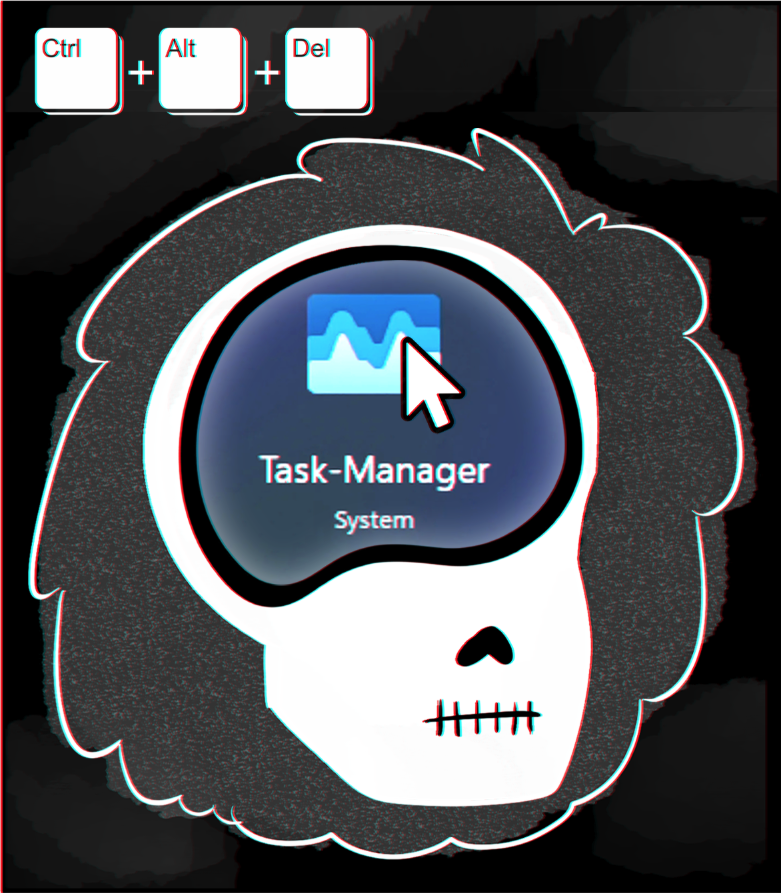
\includegraphics[width=0.8\linewidth,height=\textheight,keepaspectratio]{figures/CAD.png}

}

\caption{Ctrl + Alt + Del your distractions for academic success}

\end{figure}%

\newpage

\subsection{Problem introduction}\label{problem-introduction}

\begin{itemize}
\item
  Academic performance is affected by daily habits like:
\item
  Study hours per day, Classroom attendance, Sleep hours
\item
  On the other hand, spending too much time on:
\item
  Social media, Streaming platforms like Netflixmay reduce focus and
  study time.
\item
  Research Objective:Quantify the relationship between student habits
  and academic performance using correlation analysis.
\item
  We aim to discover which habits support academic success and which
  habits hinder it.
\end{itemize}

\newpage

\subsection{Dataset description}\label{dataset-description}

\begin{itemize}
\item
  The dataset includes \textbf{100 students} and \textbf{16 variables}
  covering lifestyle habits and exam performance.
\item
  Main variables include:

  \begin{itemize}
  \item
    Study hours per day
  \item
    Class attendance (\%)
  \item
    Sleep hours
  \item
    Social media hours
  \item
    Netflix hours
  \item
    Exam score
  \end{itemize}
\end{itemize}

\begin{itemize}
\item
  Main variables are grouped into:

  \begin{itemize}
  \tightlist
  \item
    \textbf{Good habits:}\\
    \texttt{StudyHours}, \texttt{AttendanceRate}, \texttt{SleepHours}
  \item
    \textbf{Bad habits:}\\
    \texttt{SocialMediaHours}, \texttt{NetflixHours}
  \end{itemize}
\item
  Target variable:\\
  \texttt{ExamScore} (numeric score for student performance)
\item
  Data was cleaned and renamed for clarity before analysis.
\end{itemize}

\newpage

\subsection{Methods}\label{methods}

\subsubsection{Analysis method}\label{analysis-method}

\textbf{Correlational analysis} used to test how student lifestyle
habits relate to academic performance

\subsection{Technique}\label{technique}

\begin{itemize}
\tightlist
\item
  \textbf{Pearson correlations} drawn using \texttt{cor()} in R
\item
  Created \textbf{bubble-style} plots using \texttt{corrplot()} to
  visualize magnitude and direction of relationships {Blue} = positive\\
  {Red} = negative\\
  Circle size = strength
\end{itemize}

\subsection{Table 1: Good Habits Correlation
Table}\label{table-1-good-habits-correlation-table}

\begin{longtable}[]{@{}lrrrr@{}}
\toprule\noalign{}
& StudyHours & AttendanceRate & SleepHours & ExamScore \\
\midrule\noalign{}
\endhead
\bottomrule\noalign{}
\endlastfoot
StudyHours & 1.00 & 0.03 & -0.03 & 0.83 \\
AttendanceRate & 0.03 & 1.00 & 0.01 & 0.09 \\
SleepHours & -0.03 & 0.01 & 1.00 & 0.12 \\
ExamScore & 0.83 & 0.09 & 0.12 & 1.00 \\
\end{longtable}

\subsection{Table 2: Bad Habits Correlation
Table}\label{table-2-bad-habits-correlation-table}

\begin{longtable}[]{@{}lrrr@{}}
\toprule\noalign{}
& SocialMediaHours & NetflixHours & ExamScore \\
\midrule\noalign{}
\endhead
\bottomrule\noalign{}
\endlastfoot
SocialMediaHours & 1.00 & 0.01 & -0.17 \\
NetflixHours & 0.01 & 1.00 & -0.17 \\
ExamScore & -0.17 & -0.17 & 1.00 \\
\end{longtable}

\newpage

\subsection{Results}\label{results}

\begin{itemize}
\tightlist
\item
  \textbf{Study hours} shows a \textbf{strong positive correlation} with
  exam scores
\end{itemize}

\begin{figure}[H]

{\centering \pandocbounded{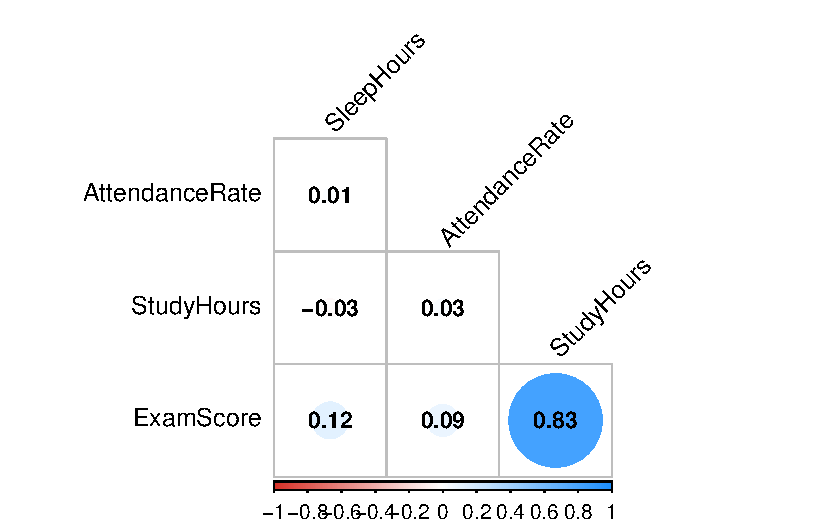
\includegraphics[keepaspectratio]{slides_files/figure-pdf/bubble-corrplot-1.pdf}}

}

\caption{Bubble-style correlation matrix of student habits and exam
score}

\end{figure}%

\newpage

\subsection{Results Continued}\label{results-continued}

\begin{itemize}
\tightlist
\item
  \emph{Social media hours} and \emph{Netflix hours} show only
  \textbf{weak negative correlation} with exam scores
\item
  \emph{Attendance rate} and \emph{Sleep hours} also show only
  \textbf{weak positive correlation} with exam scores
\end{itemize}

\begin{figure}[H]

{\centering \pandocbounded{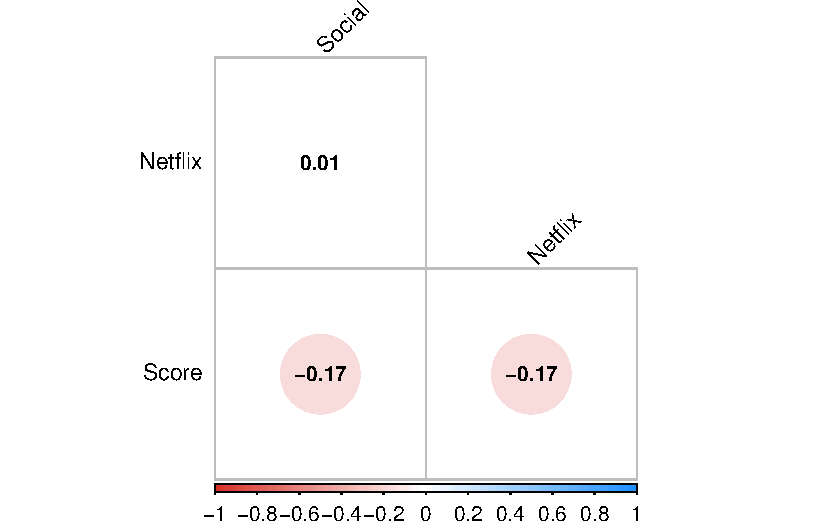
\includegraphics[keepaspectratio]{slides_files/figure-pdf/badhabits-corrplot-1.pdf}}

}

\caption{Bubble-style correlation matrix of student habits and exam
score}

\end{figure}%

\newpage

\subsection{Conclusions \&
Recommendations}\label{conclusions-recommendations}

\begin{itemize}
\item
  \textbf{StudyHours} has a \textbf{strong positive correlation} with
  ExamScore (r = 0.83).
\item
  \textbf{AttendanceRate} (r = 0.09) and \textbf{SleepHours} (r = 0.12)
  show \textbf{weak positive links}.
\item
  \textbf{SocialMediaHours} and \textbf{NetflixHours} each have a
  \textbf{weak negative correlation} (r = -0.17) with scores.
\item
  These results suggest \textbf{study time is the most reliable
  predictor} of academic success.
\end{itemize}




\end{document}
